\section{Dataset}
The data we used was obtained from a deployment of sensors in a 12-story office building
on the campus of the University of Tokyo~\cite{gutp, ogawa:lncs2011}.  The deployment consists of 
almost 700 sensors monitoring device power consumption, ranging from plug-load devices to components of the
heating, ventilation, air conditioning system and lighting.  Sensors also reported temperature
data, pressure, device-state, and other device information.  Each sensor reports data on the
order of minutes.  However, with the number of sensors, the collected data over a 2-year
span was about half a terabyte.


\begin{figure*}[tb]
\hspace{-2cm}
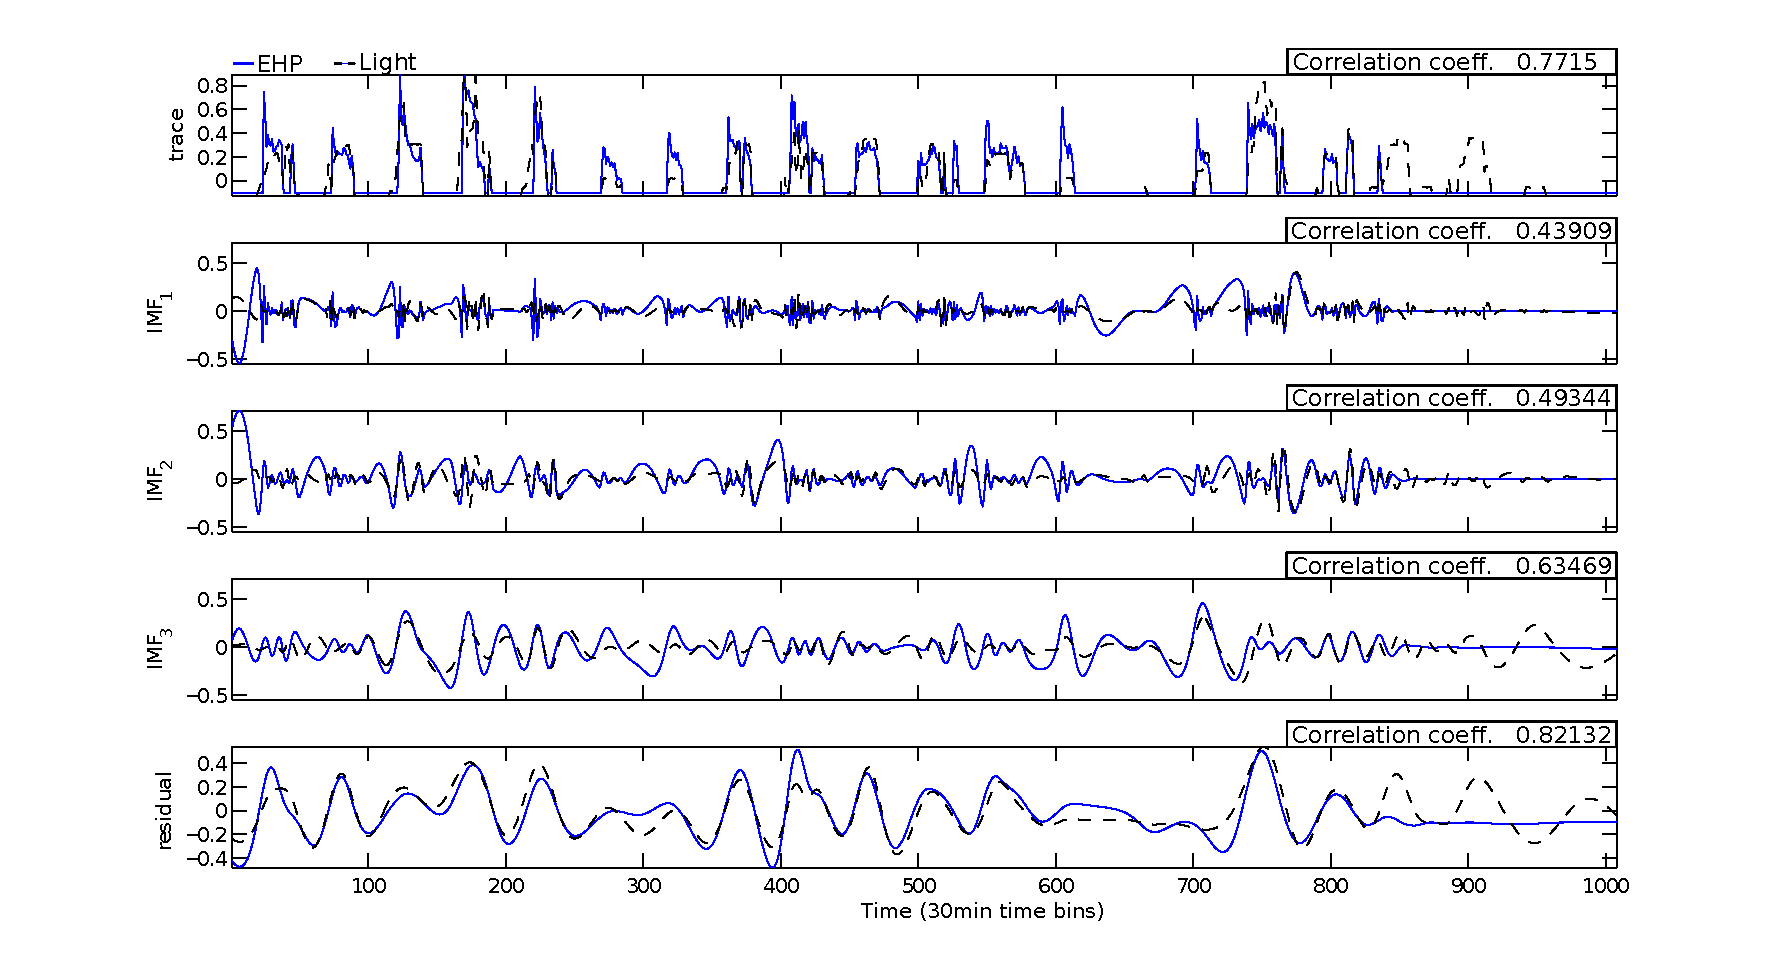
\includegraphics[width=1.2\textwidth]{img/emd_25_26-eps-converted-to}
\vspace{-1cm}
\caption{Decomposition of the EHP and light trace using bivariate EMD. Correlation coefficients highlight the intrinsic relationship of the two traces.}
\label{fig:emd}
\end{figure*}

% The intent of the Green University of Tokyo Project (GUTP) \cite{gutp} is to reduce the university environmental impacts associated to its electric energy consumption.
% The first step of this project was to deploy sensors at the Building No.2 of the Faculty of Engineering 
% Electric power consumption of a 12 floors building containing researchers office and classroom.
% 1215 sensors monitoring different devices...

%received attention in the past \cite{ogawa:lncs2011}.

For our investigation we focus on a three-week span in the summer of 2011 (from July 4th to July 24th).
The dataset capture regular work days, weekends and one holiday (July 18th).  This gave us a representative sample
of how the equipment is used for various activities as they are influenced by occupant schedules.  For the initial
analysis we also narrowed the search down to three sensors:

% includes one day holiday (July 18th)
% 3 different sensors:
\begin{itemize}
 \item Two are measuring the electric power consumption of two devices from the same room; an electric heat 
 		pump (EHP) and the room lighting system.
 \item One is measuring the electric power consumption of a gas heat pump (GHP) that is pumping water to cool 
 		a different room in the same building.
\end{itemize}

Later we expand our analysis to include all the sensors in the building.








\section{Problem statement and Initial approach}\label{problem}
In our analysis, we are focused on finding devices that are correlated in their use over time.  Therefore, the
main objective is to examine how device traces relate to one another.  The wish to identify
correlated device-trace patterns at large spatio-temporal scales.  
Figure \ref{fig:raw} shows the raw traces for the 3 devices discussed in the previous section.
Notice the common pattern in each of the traces.  The lights and pumps are on during the day and off at night.
During weekends and holidays less power is drawn.  The correlation coefficient for 
 the EHP and light is $0.7715$ while the correlation coefficient for the EHP and GHP is $0.6370$.
Running simple correlation across these traces yields high correlation coefficients between them.

% Usual measures on sensor data like correlation coefficient or granger causality \cite{kim:buildsys2010}
% -- this is not working

\begin{figure}[t!]
\centering
 \subfigure[EHP trace]{\label{fig:raw_ehp}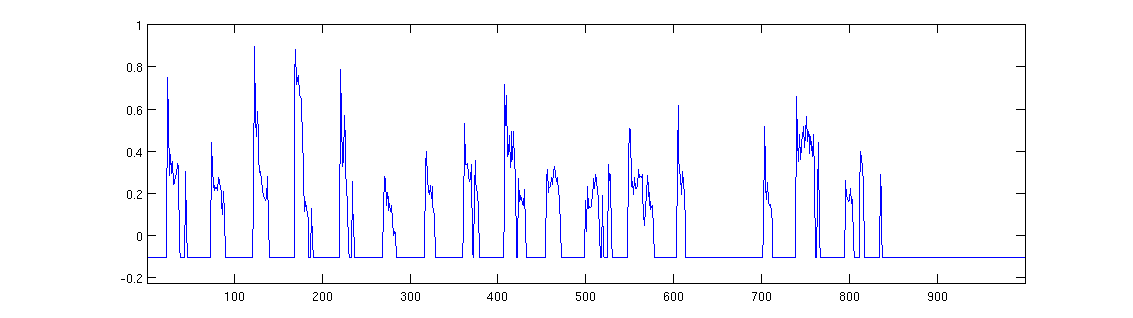
\includegraphics[width=.4\textwidth]{img/25.png}}
 \subfigure[Light trace]{\label{fig:raw_light}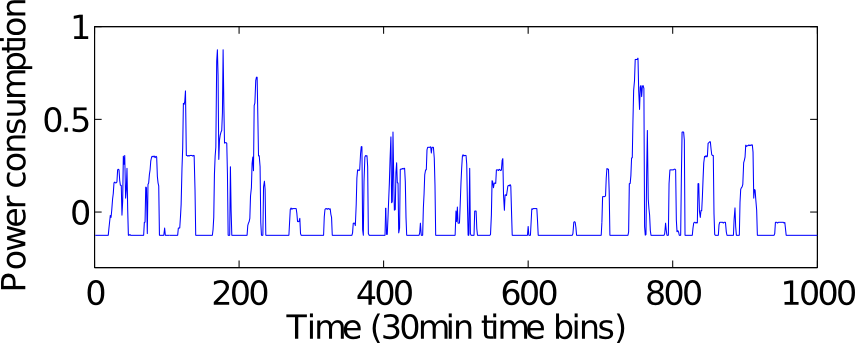
\includegraphics[width=.4\textwidth]{img/26.png}}
 \subfigure[GHP trace]{\label{fig:raw_ghp}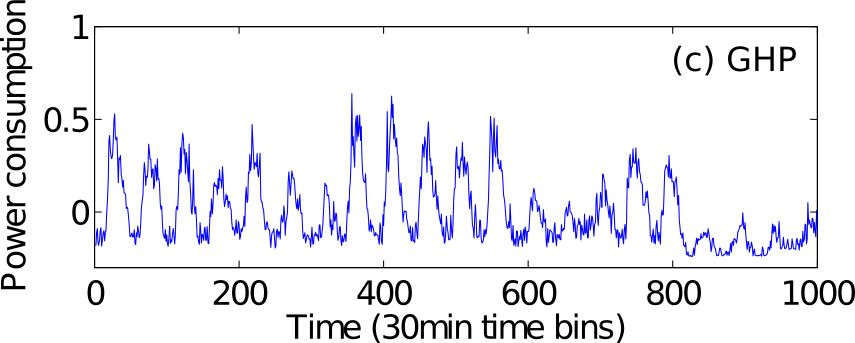
\includegraphics[width=.4\textwidth]{img/41.png}}
 \caption{Traces from three different sensors captured in 2011 from July 4th to July 24th. Data is normalized and aggregated into 30 minutes time bins.}
 \label{fig:raw}
\end{figure}

% For example correlation coefficients for the 3 signals...
% correlation coefficient for the EHP and Light signals: $0.772013$
% correlation coefficient for the EHP and GHP signals: $0.636967$

% These scores suggest that the EHP signal is related to the two other measured signals.

These results were expected for the EHP and light traces, as the two measured devices operate for the same room 
and are used simultaneously.  More importantly, they are used to support the occupants of the rooms they are serving.
We were somewhat surprised by the magnitude of correlation between the pumps, since they serve rooms on
opposite sides of the building and operate independently.  However, occupancy and weather patterns are similar,
and the underlying trend is captured by the correlation calculation.
The difference between the correlation coefficients is small and one might conclude that all three are
closely related to one another.  That conclusion is not false but misleading.  Correlation on the raw 
traces is sensitive to the underlying trend shared by the traces.  In order to meaningfully distinguish between
truly related devices we need to remove the common trends.  
% Correlation on the raw signal is not discriminatory enough.


% \begin{table}
% \begin{center}
% \begin{tabular}{|l|l|l|l|l|l|}
% \hline
% × & Raw trace & 1st IMF & 2nd IMF & 3rd IMF & Residual\\ \hline
% EHP, Light & 0.7715 & 0.43909 & 0.49344 & 0.63469 & 0.82132 \\ \hline
% EHP, GHP & 0.6370 & 0.0060274 & 0.063546 & 0.16764 & 0.79378 \\ \hline
% \end{tabular}
% \caption{Correlation coefficients of the analyzed trace and their IMFs uncovered by EMD}
% \label{tab:corr}
% \end{center}
% \end{table}
% \subsection{Simple Scenario}

\begin{figure*}[tb]
\hspace{-2cm}
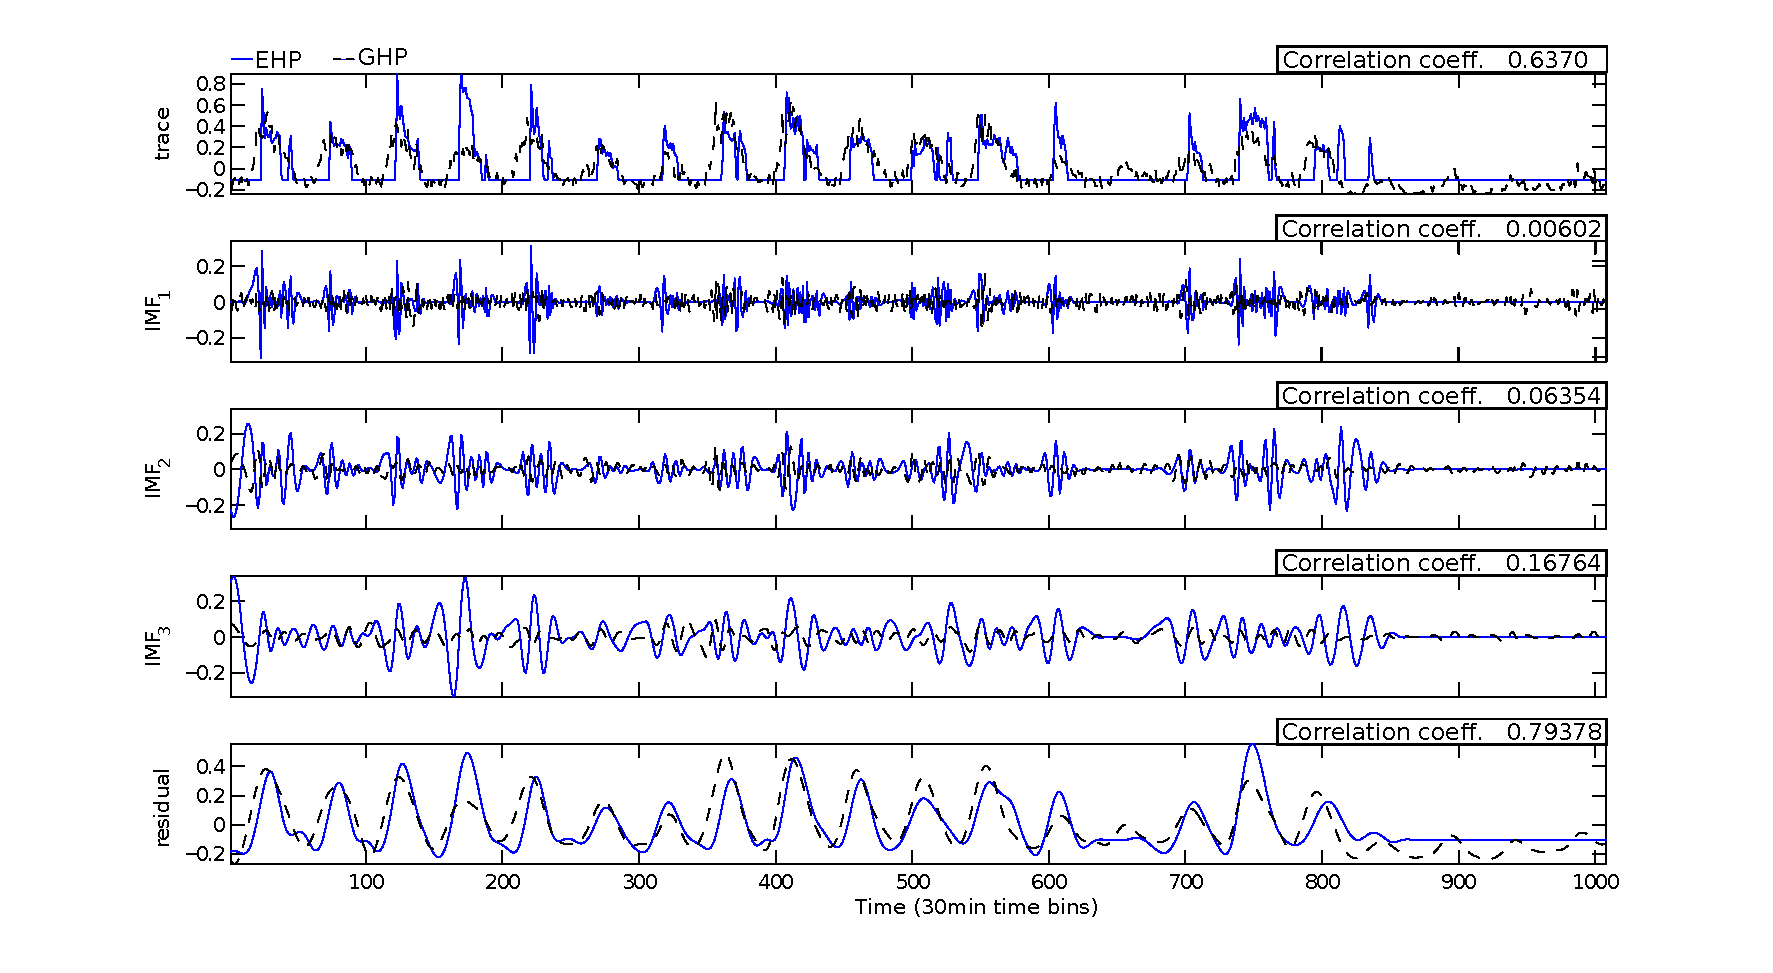
\includegraphics[width=1.2\textwidth]{img/emd_25_41-eps-converted-to}
\vspace{-1cm}
\caption{Decomposition of the EHP and GHP trace using bivariate EMD. Correlation coefficients highlight the intrinsic independence of the two traces.}
\label{fig:emd2}
\end{figure*}

% The small difference between the two computed correlation coefficients is misleading as one could conclude that the three signals are correlated and the corresponding devices are activated by a single action.

% The high correlation coefficients obtained for these three signals result .... weekly pattern....
% small difference = local fluctuation...

% this high score comes from the fact that the two devices are monitoring offices that are weekly used.

% Indeed the weekly pattern of the data trump the correlation coefficients....

% How to inspect only the local fluctuations...?
% we'd like to have an elegant solution (i.e. not specifying the interesting time scale)

